In this section we present a small performance evaluation of our algorithm.
The experiments were conducted on an AMD-6300 Six core machine with 16GB of RAM.
All the computations were executed in memory.
We have used a real world data set of hospital records from US Department of Health and Human Services.
It has 19 attributes and we designed 9 FDs for it.
We varied the number of tuples to test the scalability of our algorithm.
Figure \ref{fig:chart_2} shows the running time of generating a single repair when number of tuples in the dataset were changed from 1,000 to 100,000 tuples.
We also tested the precision of the repairs generated by our algorithm, we used the same dataset with 10,000 tuples and ran the algorithm 500 times, because we get random repair at each run.
Figure \ref{fig:chart_1} shows the variation in precision with number of changed cells in the repair.


\begin{figure}
   \centering
   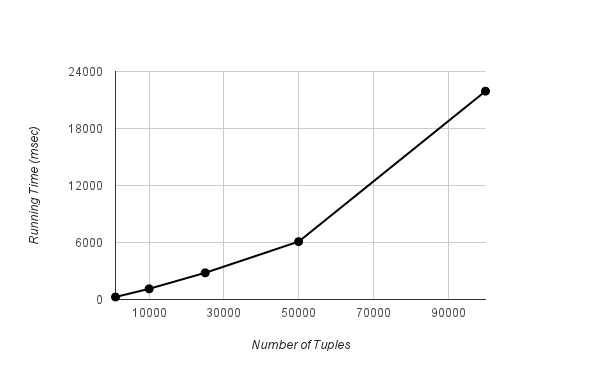
\includegraphics[scale=0.33]{chart_2.png}
   \caption{Running time of generating a repair.}
   \label{fig:chart_2}
\end{figure}

\begin{figure}
   \centering
   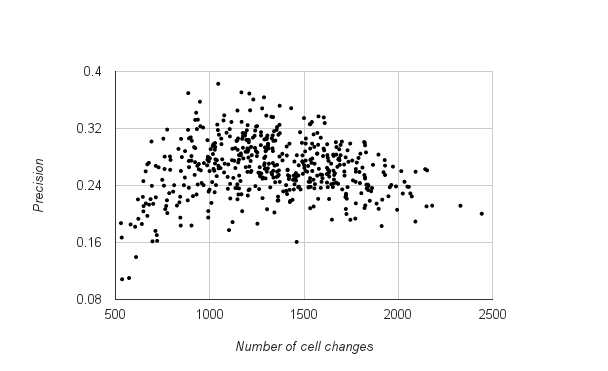
\includegraphics[scale=0.33]{chart_1.png}
   \caption{Precision variation with number of changed cells.}
   \label{fig:chart_1}
\end{figure}


